\documentclass[12pt]{article}
\usepackage{latexsym}
\usepackage{fancyhdr}
\usepackage{amssymb,amsmath,amsthm}
\usepackage[pdftex]{graphicx}
\usepackage{pdfpages}
\usepackage[margin=1in]{geometry}


% Create answer counter to keep track of seperate responses
\newcounter{AnswerCounter}
\newcounter{SubAnswerCounter}
\setcounter{AnswerCounter}{1}
\setcounter{SubAnswerCounter}{1}

% Create answer environment which uses counter
\newenvironment{answer}[0]{
  \setcounter{SubAnswerCounter}{1}
  \bigskip
  \textbf{Solution \arabic{AnswerCounter}}
  \\
  \begin{small}
}{
  \end{small}
  \stepcounter{AnswerCounter}
}

\newenvironment{subanswer}[0]{
  (\alph{SubAnswerCounter})
}{
 \bigskip
  \stepcounter{SubAnswerCounter}
}

% Allows easy use of vectors
\newcommand{\vect}[1]{\vec{\boldsymbol{#1}}}

% Setting up the title
\title{Mathematics 131 \\
Topology I}
\author{
        Luis Antonio Perez \\
        HUID: 70871564 \\
        Harvard College \\
        \href{mailto:luisperez@college.harvard.edu}{luisperez@college}
}
\date{\today}

% Custom Header information on each page
\pagestyle{fancy}
\lhead{HUID: 70871564}
\rhead{Perez - \thepage}
\renewcommand{\headrulewidth}{0.1pt}
\renewcommand{\footrulewidth}{0.1pt}

% Title page is page 0
\setcounter{page}{0}

\begin{document}
\begin{answer}[Page 425, \#1]
We show that if $G = G_1 * G_2$, then $G/[G,G] \tilde{=} (G_1 / [G_1, G_2) \oplus (G_2/[G_2, G_2])$.
\begin{proof}
We ignore the hint, instead constructing the specified homomorphisms directly. First note that $G/[G, G]$, $G_1/[G_1,G_1]$, and $G_2 / [G_2, G_2]$ are abelian, by Lemma 69.3 in Munkres. Then define the homomorphism $\Phi: G/[G,G] \to G_1/[G_1,G_1] \oplus G_2/[G_2,G_2]$, as follows:
$$
xy[G,G] \mapsto x[G_1,G_1] + y[G_2,G_2]
$$
where $x \in G_1, y \in G_2$ which must be the case because $G = G_1 * G_2$.
Note that using the extension property, the above is well-defined and is clearly a surjective homomorphism. Now we just need to show that $\Phi$ is injective. First, let us be clear about the identity elements for each group.
$$
0_{G/[G,G]} = [G,G], 0_{G_1/[G_1,G_1]} = [G_1,G_1], 0_{G_2/[G_2,G_2]} = [G_2,G_2]
$$
Assume that $xyx^{-1}y^{-1} \mapsto [G_1, G_1] \oplus [G_2, G_2]$, with $xx^{-1} \in [G_1,G_1] \subset [G,G]$ and $yy^{-1} \in [G_2,G_2] \subset [G,G]$, so using the fact the the groups are abelian:
$$
xyx^{-1}y^{-1}[G,G] = xx^{-1}yy^{-1}[G,G] = [G,G] = 0_{G/[G,G]}
$$
Following similar logic, we have that if $\prod_i x_iy_i[G,G] \to [G_1,G_1] \oplus [G_2,G_2]$, using abelian properties:
$$
\prod_i x_i \in [G_1,G_1] \subset [G,G], \prod_i y_i \in [G_2,G_2] \subset [G,G]
$$
which simplifies to:
$$
\prod_i x_iy_i[G,G] = \left( \prod_i x_i \right)\left( \prod_i y_i \right)[G,G] = [G,G]
$$
Therefore, $\Phi$ must be injective, and is the desired isomorphism.
\end{proof}
Therefore $\Phi$ are injective, which defines the desired isomorphism.
\end{answer}

\begin{answer}[Page 425, \#4]
We show that if $G = G_1 \oplus G_2$, where $G_1,G_2$ are cyclic of orders $m,n$, respectively, then $m$  and $n$ are not uniquely determined by $G$ in general.
\begin{proof}
Following the hint, suppose $m,n$ are relatively prime. Then the order of $G$ is clearly $mn$. Consider an element $g = g_1 + g_2 \in G$ where $g_1,g_2$ are the generators of $G_1,G_2$ respectively. First, we have $mng = mn(g_1 + g_2) = mng_1 + mng_2 = n(mg_1) + m(ng_2) = n0 + m0 = 0$. Therefore, it must be the case that the order $d$ of $g$ must divide $mn$. Because $m,n$ are relative prime, it must be the case that $d = mn$. This implies that the order $d$ does not always directly determine the orders $m,n$ of $G_1,G_2$.
\end{proof}
\end{answer}

\begin{answer}[Page 433, \#1]
We suppose that the homomorphism $i_*$ induced by inclusion $i: U \cap V \to X$ is trivial. We will reference Diagram throughout this question.
\begin{figure}[h!]
\centering
\caption{Homomorphism Diagram}
\label{diag:homomorphisms}
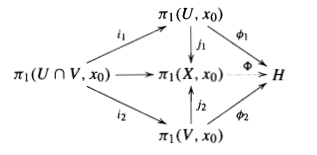
\includegraphics{map_diagram.png}
\end{figure}
\begin{itemize}
\item We show that $j_1, j_2$ induces an epimorphism:
$$
h: (\pi_1(U,x_0)/N_1) * (\pi_1(V,x_0)/N_2) \to \pi_1(X,x_0)
$$
where $N_1$ is the least normal subgroup of $\pi_1(U,x_0)$ containing image $i_1$ and $N_2$ is the least normal subgroup of $\pi_1(V,x_0)$ containing image $i_2$.
\begin{proof}
First note that $i_* = j_1 \circ i_1$ and $i_* = j_2 \circ i_2$. Therefore, the image of $i_1$ is contained in both the $\text{ker}(j_1)$ and in $N_1$, and the image of $i_2$ is contained in both the $\text{ker}(j_2)$ and in $N_2$. This implies that $N_1$ is a subgroup of $\text{ker}(j_1)$, and similarly, $N_2$ is a subgroup of $\text{ker}(j_2)$. (They are both the least normal subgroups). Therefore, it must be possible to find homomorphisms $h_1: \pi_1(U,x_0)/N_1 \to \pi_1(X,x_0)$ and $h_2: \pi_1(V,x_0)/N_2 \to \pi_1(X,x_0)$ such that $j_1 = h_1 \circ \text{proj}_{\pi_1(U,x_0)/N_1}$ and $j_2 = h_2 \circ \text{proj}_{\pi_1(V,x_0)/N_2}$ since we lose no information in the projection that wouldn't have been lost by $j_*$ already. Then we can define:
$$
h: \pi_1(U,x_0)/N_1 * \pi_1(V,x_0)/N_1 \to \pi_1(X,x_0)
$$
as the extension of $h_1,h_2$ to the free product. Then consider the map induced by inclusions $j: \pi_1(U,x_0) * \pi_2(V,x_0) \to \pi(X,x_0)$, and note that it is an epimorphism (onto map). Then note, additionally, that we can write $j = h \circ \text{proj}_{\pi_1(U,x_0)/N_1 * \pi_1(V,x_0)/N_2}$ without loss of information. Therefore, $h$ must also be an epimorphism, as desired.
\end{proof}
\item We show that $h$ is an isomorphism.
\begin{proof}
We make use of Theorem 70.1. Let the assumptions of the theorem hold, with $H = \pi_1(U,x_0)/N_1 * \pi_2(V,x_0)/N_2$. Then note that $\phi_1$ is defined as the coset projection of $\pi(U,x_0)$ followed by inclusion into the free product. Similarly for $\phi_2$. And lastly, note that the equation $\phi_1 \circ i_i = \phi_2 \circ i_2$ is satisfied, as it is the coset projection of the intersection followed by inclusion. By Theorem 70.1, there exists a unique homomorphism $\Phi: \pi_1(X,x_0) \to  \pi_1(U,x_0)/N_1 * \pi_2(V,x_0)/N_2$ such that $\Phi \circ j_1 = \phi_1$ and $\Phi \circ j_2 = \phi_2$. We claim that $\Phi$ is the left inverse of $h$. To see this, note:
\begin{align*}
\Phi \circ h \circ \phi_1 &= \Phi \circ h \circ \text{inclusion}_{\pi_1(U,x_0)/N_1 * \pi_1(V,x_0)/N_2} \circ \text{proj}_{\pi_1(U,x_0)/N_1} \tag{definition of $\phi_1$} \\
&= \Phi \circ h_1 \circ \text{proj}_{\pi_1(U,x_0)/N_1} \tag{definition of $h$ as extension of $h_1,h_2$} \\
&= \Phi \circ j_1 \tag{see above} \\
&= \phi_1 \tag{definition of $\phi_1$}
\end{align*}
Similarly, for $\phi_2$ we have that $\Phi \circ h \circ \phi_2 = \phi_2$. Combining these two results with the fact that $\pi_1(U,x_0)/N_1 * \pi_1(V,x_0)/N_1$ is generated by $im (\phi_1)$ and $im(\phi_2)$, we must have that $\Phi \circ h = id$. Therefore, $\Phi$ is the left inverse of $h$, so $h$ must be injective. Combined with the results from above, this means that $h$ is an isomorphism.
\end{proof}
\end{itemize}
\end{answer}

\begin{answer}[Page 438, \#2]
We let $X$ be a space that is the union of closed subspaces $X_1, \cdots, X_n$, and let $p \in X$ be a point such that $X_1 \cap X_j = \{p\}$ for $i \neq j$.Then we call $X$ the wedge of the spaces $X_1, \cdots X_n$ and write $X = X_1 \lor \cdots \lor X_n$. We show that if for each $i$ the point $p$ is a deformation retract of an open set $W_i$ of $X_i$, then $\pi_1(X,p)$ is the external product of the groups $\pi_1(X_i,p)$ relative to the monomorphisms induced by inclusions.
\begin{proof}
The proof follows a format similar to Theorem 71.1. We proof by induction. Note that for the case of $n= 1$, the result follow trivially. \\

Now, let $X$ be the wedge of the spaces $X_1, \cdots, X_k$ with $p$ the common point. Then define the following two sets:
\begin{align*}
U &= X_1 \cup W_2 \cup \cdots \cup W_n \\
V &= W_1 \cup X_2 \cup \cdots X_n
\end{align*}
Then note that $U \cap V = W_1 \cup \cdots \cup W_n$. Let $F_i: W_i \times I \to W_i$ be the deformation retraction. The maps $F_i$ fit together to define a map $F: (U \cap V) \times I \to U \cap V$ that is a deformation retraction of $U \cap V$ onto $p$. To show continuity, note that $W_i$ are closed subspaces of $U \cap V$, so that $W_i \times I$ is a closed subspace of $(U \cap V) \times I$. Then the pasting lemma applies). It follows from this that $U \cap V$ is simply connected, so that $\pi_1(X,p)$ is the free product of the groups $\pi_1(U,p)$ and $\pi_1(V,p)$, relative to the mono-morphisms induced by inclusion. This implies that it is the external free product of these groups. \\

By a similar argument, note that the maps fit together to form $F_U: U \to U$, a reformation retract of $U$ onto $X_1$. Similarly, $X_2 \cup \cdots \cup X_n$ is a deformation retract of $V$. From this, it follows that $\pi_1(U,p)$ is is equivalent to $\pi_1(X_1,p)$. By the inductive hypothesis, it also follows that $\pi_1(V,p)$ is a the external product of the groups $\pi_1(X_2,p),\cdots, \pi_1(X_n,p)$. Therefore, we have that $\pi_1(X,p)$ is the external product of $\pi_1(X_i,p)$.
\end{proof}
\end{answer}

\begin{answer}[Page 445, \#1]
We find spaces whose fundamental groups are isomorphic to the following groups (where $\mathbb{Z}/n$ denote the additive group of integers modulo $n$).
\begin{enumerate}
\item $\mathbb{Z}/n \times \mathbb{Z}/m$: We let $X_n$ be the $n$-fold dunce cap and $X_m$ be the $m$-fold dunce cap. Then by Theorem 73.4, $\pi_1(X_n,x_0) \tilde{=} \mathbb{Z}/n$ and $\pi_1(X_m,x_1) \tilde{=} \mathbb{Z}/m$. Therefore, we let $X = X_1 \times X_2$. Then $\pi_1(X,(x_0,x_1)) \tilde{=} \pi_1(X_n,x_1) \times \pi_1(X_m,x_1) \tilde{=} \mathbb{Z}/n \times \mathbb{Z}/m$.
\item We can immediately see by induction on the above, that the space we need is $X = X_1 \times X_{n_{2}} \times  \cdots \times X_{n_k}$. Where $X_{n_i}$ is the $n_i$-fold dunce cap.
\item Using the results from Exercise 2 of Section 71, we can again let $X_n, X_m$ be the $n$ and $m$-fold dunce caps, respectively. Then by the results from Exercise 2 of Section 71, $\pi_1(X_n \lor X_m, x_0) \tilde{=} \pi_1(X_n,x_0) * \pi_1(X_m,x_0) \tilde{=} \mathbb{Z}/n \times \mathbb{Z}/m$.
\item Using the results from above, and by the fact the free product is associative, we can use induction to show that the space we need is $X = X_{n_1} \lor X_{n_2} \lor \cdots \lor X_{n_k}$ because then we have $\pi_1(X,x_0) \tilde{=} \pi_1(X_{n_1}, x_0) * \pi_1(X_{n_2},x_0) * \cdots * \pi_1(X_{n_k},x_0) \tilde{=} \mathbb{Z}/n_1 * \mathbb{Z}/n_2 * \cdots * \mathbb{Z}/n_k$.
\end{enumerate}
\end{answer}

\end{document}